\documentclass{standalone}
\usepackage{tikz}
\usetikzlibrary{patterns, positioning}


\begin{document}
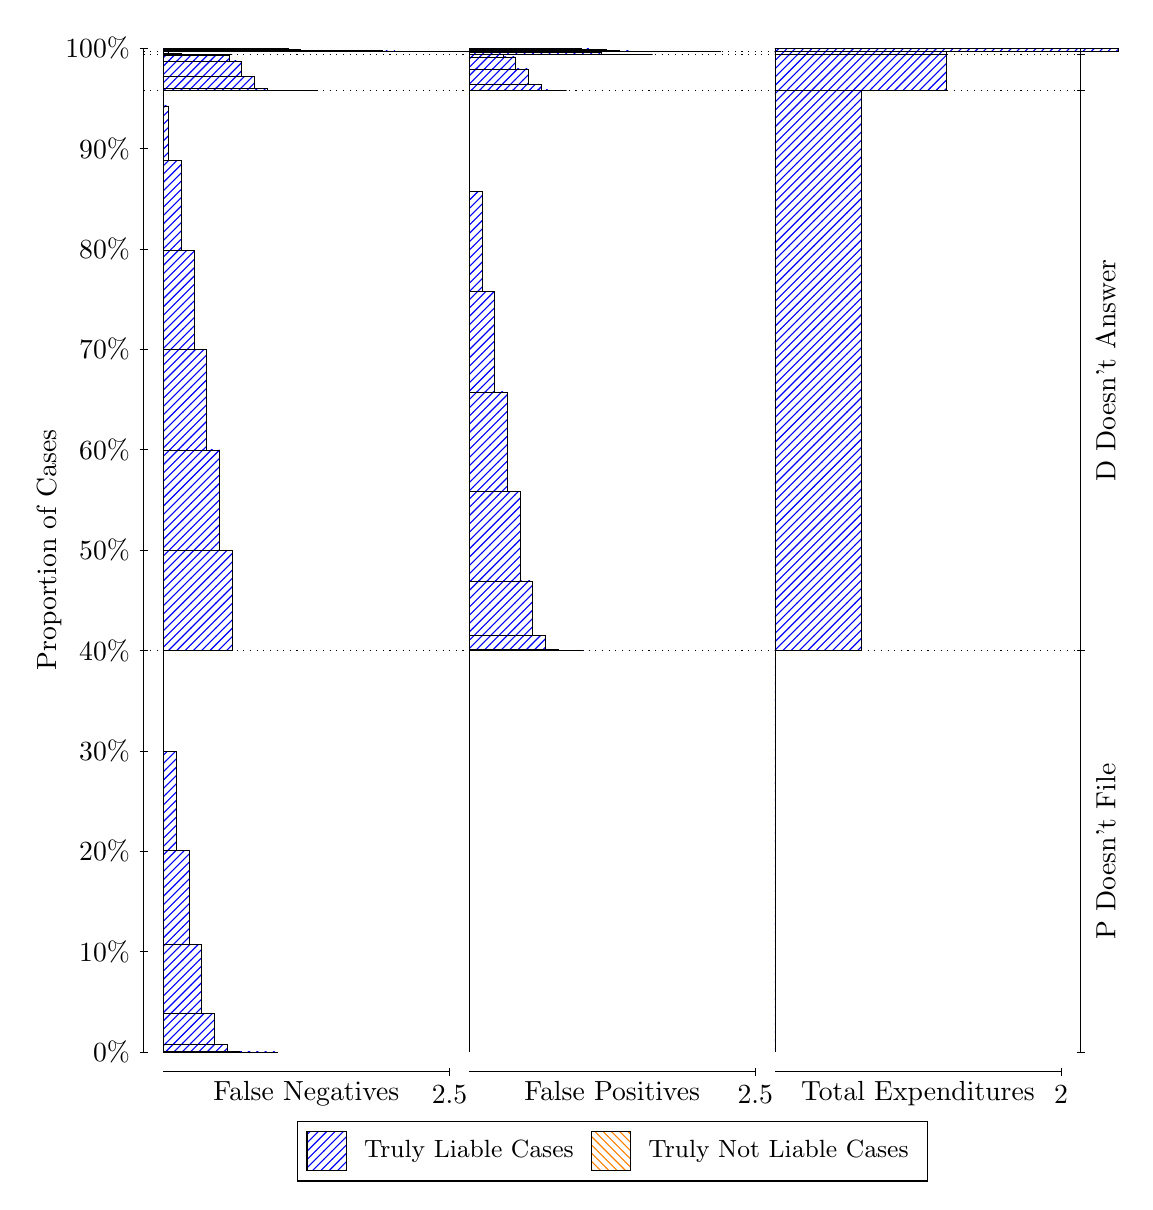
\begin{tikzpicture}
\draw[black, very thin] (1.5,1.75) -- (1.5,14.5);
\node[rotate=90, text=black, anchor=center] at (0.3, 8.125) {Proportion of Cases};
\draw[black, very thin] (1.45,1.75) -- (1.55,1.75);
\node[text=black, anchor=east] at (1.45, 1.75) {0\%};
\draw[black, very thin] (1.45,3.025) -- (1.55,3.025);
\node[text=black, anchor=east] at (1.45, 3.025) {10\%};
\draw[black, very thin] (1.45,4.3) -- (1.55,4.3);
\node[text=black, anchor=east] at (1.45, 4.3) {20\%};
\draw[black, very thin] (1.45,5.575) -- (1.55,5.575);
\node[text=black, anchor=east] at (1.45, 5.575) {30\%};
\draw[black, very thin] (1.45,6.85) -- (1.55,6.85);
\node[text=black, anchor=east] at (1.45, 6.85) {40\%};
\draw[black, very thin] (1.45,8.125) -- (1.55,8.125);
\node[text=black, anchor=east] at (1.45, 8.125) {50\%};
\draw[black, very thin] (1.45,9.4) -- (1.55,9.4);
\node[text=black, anchor=east] at (1.45, 9.4) {60\%};
\draw[black, very thin] (1.45,10.675) -- (1.55,10.675);
\node[text=black, anchor=east] at (1.45, 10.675) {70\%};
\draw[black, very thin] (1.45,11.95) -- (1.55,11.95);
\node[text=black, anchor=east] at (1.45, 11.95) {80\%};
\draw[black, very thin] (1.45,13.225) -- (1.55,13.225);
\node[text=black, anchor=east] at (1.45, 13.225) {90\%};
\draw[black, very thin] (1.45,14.5) -- (1.55,14.5);
\node[text=black, anchor=east] at (1.45, 14.5) {100\%};

\draw[black, very thin] (13.4,1.75) -- (13.4,14.5);
\draw[black, very thin] (13.35,1.75) -- (13.45,1.75);
\node[anchor=west] at (13.35, 1.75) {};
\draw[black, very thin] (13.35,6.8465) -- (13.45,6.8465);
\node[anchor=west] at (13.35, 6.8465) {};
\draw[black, very thin] (13.35,13.959) -- (13.45,13.959);
\node[anchor=west] at (13.35, 13.959) {};
\draw[black, very thin] (13.35,14.417) -- (13.45,14.417);
\node[anchor=west] at (13.35, 14.417) {};
\draw[black, very thin] (13.35,14.458) -- (13.45,14.458);
\node[anchor=west] at (13.35, 14.458) {};
\draw[black, very thin] (13.35,14.5) -- (13.45,14.5);
\node[anchor=west] at (13.35, 14.5) {};

\draw[black, very thin, pattern color=blue, pattern=north east lines] (1.75,1.75) rectangle (3.2033,1.75);
\draw[black, very thin, pattern color=blue, pattern=north east lines] (1.75,1.75) rectangle (3.0419,1.75);
\draw[black, very thin, pattern color=blue, pattern=north east lines] (1.75,1.75) rectangle (2.8804,1.7503);
\draw[black, very thin, pattern color=blue, pattern=north east lines] (1.75,1.7503) rectangle (2.7189,1.7582);
\draw[black, very thin, pattern color=blue, pattern=north east lines] (1.75,1.7582) rectangle (2.5574,1.8433);
\draw[black, very thin, pattern color=blue, pattern=north east lines] (1.75,1.8433) rectangle (2.3959,2.2362);
\draw[black, very thin, pattern color=blue, pattern=north east lines] (1.75,2.2362) rectangle (2.2344,3.1169);
\draw[black, very thin, pattern color=blue, pattern=north east lines] (1.75,3.1169) rectangle (2.073,4.3056);
\draw[black, very thin, pattern color=blue, pattern=north east lines] (1.75,4.3056) rectangle (1.9115,5.572);
\draw[black, very thin, pattern color=orange, pattern=north west lines] (1.75,5.572) rectangle (1.75,5.572);
\draw[black, very thin, pattern color=blue, pattern=north east lines] (1.75,5.572) rectangle (1.75,6.8465);
\draw[black, very thin, pattern color=blue, pattern=north east lines] (1.75,6.8465) rectangle (2.622,8.1216);
\draw[black, very thin, pattern color=blue, pattern=north east lines] (1.75,8.1216) rectangle (2.4605,9.3966);
\draw[black, very thin, pattern color=blue, pattern=north east lines] (1.75,9.3966) rectangle (2.299,10.671);
\draw[black, very thin, pattern color=blue, pattern=north east lines] (1.75,10.671) rectangle (2.1376,11.933);
\draw[black, very thin, pattern color=blue, pattern=north east lines] (1.75,11.933) rectangle (1.9761,13.072);
\draw[black, very thin, pattern color=blue, pattern=north east lines] (1.75,13.072) rectangle (1.8146,13.764);
\draw[black, very thin, pattern color=orange, pattern=north west lines] (1.75,13.764) rectangle (1.75,13.764);
\draw[black, very thin, pattern color=blue, pattern=north east lines] (1.75,13.764) rectangle (1.75,13.959);
\draw[black, very thin, pattern color=blue, pattern=north east lines] (1.75,13.959) rectangle (3.712,13.959);
\draw[black, very thin, pattern color=blue, pattern=north east lines] (1.75,13.959) rectangle (3.5505,13.959);
\draw[black, very thin, pattern color=blue, pattern=north east lines] (1.75,13.959) rectangle (3.389,13.959);
\draw[black, very thin, pattern color=blue, pattern=north east lines] (1.75,13.959) rectangle (3.2276,13.96);
\draw[black, very thin, pattern color=blue, pattern=north east lines] (1.75,13.96) rectangle (3.0661,13.988);
\draw[black, very thin, pattern color=blue, pattern=north east lines] (1.75,13.988) rectangle (2.9046,14.14);
\draw[black, very thin, pattern color=blue, pattern=north east lines] (1.75,14.14) rectangle (2.7431,14.338);
\draw[black, very thin, pattern color=blue, pattern=north east lines] (1.75,14.338) rectangle (2.5816,14.408);
\draw[black, very thin, pattern color=blue, pattern=north east lines] (1.75,14.408) rectangle (2.4201,14.416);
\draw[black, very thin, pattern color=blue, pattern=north east lines] (1.75,14.416) rectangle (2.2587,14.417);
\draw[black, very thin, pattern color=orange, pattern=north west lines] (1.75,14.417) rectangle (1.75,14.417);
\draw[black, very thin, pattern color=blue, pattern=north east lines] (1.75,14.417) rectangle (2.622,14.417);
\draw[black, very thin, pattern color=blue, pattern=north east lines] (1.75,14.417) rectangle (2.4605,14.417);
\draw[black, very thin, pattern color=blue, pattern=north east lines] (1.75,14.417) rectangle (2.299,14.417);
\draw[black, very thin, pattern color=blue, pattern=north east lines] (1.75,14.417) rectangle (2.1376,14.419);
\draw[black, very thin, pattern color=blue, pattern=north east lines] (1.75,14.419) rectangle (1.9761,14.434);
\draw[black, very thin, pattern color=blue, pattern=north east lines] (1.75,14.434) rectangle (1.8146,14.453);
\draw[black, very thin, pattern color=orange, pattern=north west lines] (1.75,14.453) rectangle (1.75,14.453);
\draw[black, very thin, pattern color=blue, pattern=north east lines] (1.75,14.453) rectangle (1.75,14.458);
\draw[black, very thin, pattern color=blue, pattern=north east lines] (1.75,14.458) rectangle (5.8193,14.458);
\draw[black, very thin, pattern color=blue, pattern=north east lines] (1.75,14.458) rectangle (5.6579,14.458);
\draw[black, very thin, pattern color=blue, pattern=north east lines] (1.75,14.458) rectangle (5.4964,14.458);
\draw[black, very thin, pattern color=blue, pattern=north east lines] (1.75,14.458) rectangle (5.3349,14.458);
\draw[black, very thin, pattern color=blue, pattern=north east lines] (1.75,14.458) rectangle (5.1734,14.458);
\draw[black, very thin, pattern color=blue, pattern=north east lines] (1.75,14.458) rectangle (5.0119,14.458);
\draw[black, very thin, pattern color=blue, pattern=north east lines] (1.75,14.458) rectangle (5.0119,14.458);
\draw[black, very thin, pattern color=blue, pattern=north east lines] (1.75,14.458) rectangle (4.8504,14.459);
\draw[black, very thin, pattern color=blue, pattern=north east lines] (1.75,14.459) rectangle (4.8504,14.46);
\draw[black, very thin, pattern color=blue, pattern=north east lines] (1.75,14.46) rectangle (4.689,14.463);
\draw[black, very thin, pattern color=blue, pattern=north east lines] (1.75,14.463) rectangle (4.5275,14.464);
\draw[black, very thin, pattern color=blue, pattern=north east lines] (1.75,14.464) rectangle (4.5275,14.466);
\draw[black, very thin, pattern color=blue, pattern=north east lines] (1.75,14.466) rectangle (4.4629,14.466);
\draw[black, very thin, pattern color=blue, pattern=north east lines] (1.75,14.466) rectangle (4.366,14.467);
\draw[black, very thin, pattern color=blue, pattern=north east lines] (1.75,14.467) rectangle (4.3014,14.467);
\draw[black, very thin, pattern color=blue, pattern=north east lines] (1.75,14.467) rectangle (4.2045,14.467);
\draw[black, very thin, pattern color=blue, pattern=north east lines] (1.75,14.467) rectangle (4.1399,14.467);
\draw[black, very thin, pattern color=blue, pattern=north east lines] (1.75,14.467) rectangle (4.043,14.467);
\draw[black, very thin, pattern color=blue, pattern=north east lines] (1.75,14.467) rectangle (3.9784,14.467);
\draw[black, very thin, pattern color=blue, pattern=north east lines] (1.75,14.467) rectangle (3.817,14.468);
\draw[black, very thin, pattern color=blue, pattern=north east lines] (1.75,14.468) rectangle (3.817,14.468);
\draw[black, very thin, pattern color=blue, pattern=north east lines] (1.75,14.468) rectangle (3.6555,14.474);
\draw[black, very thin, pattern color=blue, pattern=north east lines] (1.75,14.474) rectangle (3.6555,14.474);
\draw[black, very thin, pattern color=blue, pattern=north east lines] (1.75,14.474) rectangle (3.494,14.484);
\draw[black, very thin, pattern color=blue, pattern=north east lines] (1.75,14.484) rectangle (3.3325,14.487);
\draw[black, very thin, pattern color=blue, pattern=north east lines] (1.75,14.487) rectangle (3.3325,14.493);
\draw[black, very thin, pattern color=blue, pattern=north east lines] (1.75,14.493) rectangle (3.171,14.493);
\draw[black, very thin, pattern color=blue, pattern=north east lines] (1.75,14.493) rectangle (3.171,14.497);
\draw[black, very thin, pattern color=blue, pattern=north east lines] (1.75,14.497) rectangle (3.171,14.498);
\draw[black, very thin, pattern color=blue, pattern=north east lines] (1.75,14.498) rectangle (3.0096,14.499);
\draw[black, very thin, pattern color=blue, pattern=north east lines] (1.75,14.499) rectangle (3.0096,14.5);
\draw[black, very thin, pattern color=blue, pattern=north east lines] (1.75,14.5) rectangle (2.8481,14.5);
\draw[black, very thin, pattern color=blue, pattern=north east lines] (1.75,14.5) rectangle (2.6866,14.5);
\draw[black, very thin, pattern color=blue, pattern=north east lines] (1.75,14.5) rectangle (2.5251,14.5);
\draw[black, very thin, pattern color=blue, pattern=north east lines] (1.75,14.5) rectangle (2.5251,14.5);
\draw[black, very thin, pattern color=blue, pattern=north east lines] (1.75,14.5) rectangle (2.3636,14.5);
\draw[black, very thin, pattern color=blue, pattern=north east lines] (1.75,14.5) rectangle (2.3636,14.5);
\draw[black, very thin, pattern color=blue, pattern=north east lines] (1.75,14.5) rectangle (2.2021,14.5);
\draw[black, very thin, pattern color=blue, pattern=north east lines] (1.75,14.5) rectangle (2.2021,14.5);
\draw[black, very thin, pattern color=blue, pattern=north east lines] (1.75,14.5) rectangle (2.0407,14.5);
\draw[black, very thin, pattern color=orange, pattern=north west lines] (1.75,14.5) rectangle (1.75,14.5);
\draw[black, very thin, pattern color=orange, pattern=north west lines] (5.6333,1.75) rectangle (5.6333,1.75);
\draw[black, very thin, pattern color=blue, pattern=north east lines] (5.6333,1.75) rectangle (5.6333,6.8465);
\draw[black, very thin, pattern color=orange, pattern=north west lines] (5.6333,6.8465) rectangle (7.0867,6.8465);
\draw[black, very thin, pattern color=blue, pattern=north east lines] (5.6333,6.8465) rectangle (7.0867,6.8465);
\draw[black, very thin, pattern color=blue, pattern=north east lines] (5.6333,6.8465) rectangle (6.9252,6.8468);
\draw[black, very thin, pattern color=blue, pattern=north east lines] (5.6333,6.8468) rectangle (6.7637,6.8607);
\draw[black, very thin, pattern color=blue, pattern=north east lines] (5.6333,6.8607) rectangle (6.6022,7.0411);
\draw[black, very thin, pattern color=blue, pattern=north east lines] (5.6333,7.0411) rectangle (6.4407,7.7338);
\draw[black, very thin, pattern color=blue, pattern=north east lines] (5.6333,7.7338) rectangle (6.2793,8.8722);
\draw[black, very thin, pattern color=blue, pattern=north east lines] (5.6333,8.8722) rectangle (6.1178,10.134);
\draw[black, very thin, pattern color=blue, pattern=north east lines] (5.6333,10.134) rectangle (5.9563,11.409);
\draw[black, very thin, pattern color=blue, pattern=north east lines] (5.6333,11.409) rectangle (5.7948,12.684);
\draw[black, very thin, pattern color=blue, pattern=north east lines] (5.6333,12.684) rectangle (5.6333,13.959);
\draw[black, very thin, pattern color=orange, pattern=north west lines] (5.6333,13.959) rectangle (6.8687,13.959);
\draw[black, very thin, pattern color=blue, pattern=north east lines] (5.6333,13.959) rectangle (6.8687,13.959);
\draw[black, very thin, pattern color=blue, pattern=north east lines] (5.6333,13.959) rectangle (6.7072,13.968);
\draw[black, very thin, pattern color=blue, pattern=north east lines] (5.6333,13.968) rectangle (6.5457,14.038);
\draw[black, very thin, pattern color=blue, pattern=north east lines] (5.6333,14.038) rectangle (6.3842,14.235);
\draw[black, very thin, pattern color=blue, pattern=north east lines] (5.6333,14.235) rectangle (6.2227,14.387);
\draw[black, very thin, pattern color=blue, pattern=north east lines] (5.6333,14.387) rectangle (6.0613,14.415);
\draw[black, very thin, pattern color=blue, pattern=north east lines] (5.6333,14.415) rectangle (5.8998,14.417);
\draw[black, very thin, pattern color=blue, pattern=north east lines] (5.6333,14.417) rectangle (5.7383,14.417);
\draw[black, very thin, pattern color=blue, pattern=north east lines] (5.6333,14.417) rectangle (5.6333,14.417);
\draw[black, very thin, pattern color=orange, pattern=north west lines] (5.6333,14.417) rectangle (7.9587,14.417);
\draw[black, very thin, pattern color=blue, pattern=north east lines] (5.6333,14.417) rectangle (7.9587,14.417);
\draw[black, very thin, pattern color=blue, pattern=north east lines] (5.6333,14.417) rectangle (7.7972,14.417);
\draw[black, very thin, pattern color=blue, pattern=north east lines] (5.6333,14.417) rectangle (7.6357,14.417);
\draw[black, very thin, pattern color=blue, pattern=north east lines] (5.6333,14.417) rectangle (7.4742,14.422);
\draw[black, very thin, pattern color=blue, pattern=north east lines] (5.6333,14.422) rectangle (7.3127,14.441);
\draw[black, very thin, pattern color=blue, pattern=north east lines] (5.6333,14.441) rectangle (7.1513,14.455);
\draw[black, very thin, pattern color=blue, pattern=north east lines] (5.6333,14.455) rectangle (6.9898,14.458);
\draw[black, very thin, pattern color=blue, pattern=north east lines] (5.6333,14.458) rectangle (6.8283,14.458);
\draw[black, very thin, pattern color=blue, pattern=north east lines] (5.6333,14.458) rectangle (6.6668,14.458);
\draw[black, very thin, pattern color=blue, pattern=north east lines] (5.6333,14.458) rectangle (6.5053,14.458);
\draw[black, very thin, pattern color=orange, pattern=north west lines] (5.6333,14.458) rectangle (8.8307,14.458);
\draw[black, very thin, pattern color=blue, pattern=north east lines] (5.6333,14.458) rectangle (8.8307,14.458);
\draw[black, very thin, pattern color=blue, pattern=north east lines] (5.6333,14.458) rectangle (8.6692,14.458);
\draw[black, very thin, pattern color=orange, pattern=north west lines] (5.6333,14.458) rectangle (8.6692,14.458);
\draw[black, very thin, pattern color=blue, pattern=north east lines] (5.6333,14.458) rectangle (8.6692,14.458);
\draw[black, very thin, pattern color=orange, pattern=north west lines] (5.6333,14.458) rectangle (8.5077,14.458);
\draw[black, very thin, pattern color=blue, pattern=north east lines] (5.6333,14.458) rectangle (8.5077,14.458);
\draw[black, very thin, pattern color=blue, pattern=north east lines] (5.6333,14.458) rectangle (8.5077,14.458);
\draw[black, very thin, pattern color=blue, pattern=north east lines] (5.6333,14.458) rectangle (8.3462,14.458);
\draw[black, very thin, pattern color=orange, pattern=north west lines] (5.6333,14.458) rectangle (8.3462,14.458);
\draw[black, very thin, pattern color=blue, pattern=north east lines] (5.6333,14.458) rectangle (8.3462,14.458);
\draw[black, very thin, pattern color=blue, pattern=north east lines] (5.6333,14.458) rectangle (8.3462,14.458);
\draw[black, very thin, pattern color=blue, pattern=north east lines] (5.6333,14.458) rectangle (8.1847,14.458);
\draw[black, very thin, pattern color=orange, pattern=north west lines] (5.6333,14.458) rectangle (8.1847,14.458);
\draw[black, very thin, pattern color=blue, pattern=north east lines] (5.6333,14.458) rectangle (8.1847,14.458);
\draw[black, very thin, pattern color=blue, pattern=north east lines] (5.6333,14.458) rectangle (8.1847,14.458);
\draw[black, very thin, pattern color=blue, pattern=north east lines] (5.6333,14.458) rectangle (8.0233,14.458);
\draw[black, very thin, pattern color=orange, pattern=north west lines] (5.6333,14.458) rectangle (8.0233,14.458);
\draw[black, very thin, pattern color=blue, pattern=north east lines] (5.6333,14.458) rectangle (8.0233,14.458);
\draw[black, very thin, pattern color=blue, pattern=north east lines] (5.6333,14.458) rectangle (8.0233,14.458);
\draw[black, very thin, pattern color=blue, pattern=north east lines] (5.6333,14.458) rectangle (7.8618,14.458);
\draw[black, very thin, pattern color=blue, pattern=north east lines] (5.6333,14.458) rectangle (7.8618,14.46);
\draw[black, very thin, pattern color=orange, pattern=north west lines] (5.6333,14.46) rectangle (7.8618,14.46);
\draw[black, very thin, pattern color=blue, pattern=north east lines] (5.6333,14.46) rectangle (7.8618,14.46);
\draw[black, very thin, pattern color=blue, pattern=north east lines] (5.6333,14.46) rectangle (7.8618,14.46);
\draw[black, very thin, pattern color=blue, pattern=north east lines] (5.6333,14.46) rectangle (7.7003,14.46);
\draw[black, very thin, pattern color=blue, pattern=north east lines] (5.6333,14.46) rectangle (7.7003,14.464);
\draw[black, very thin, pattern color=blue, pattern=north east lines] (5.6333,14.464) rectangle (7.7003,14.465);
\draw[black, very thin, pattern color=blue, pattern=north east lines] (5.6333,14.465) rectangle (7.5388,14.465);
\draw[black, very thin, pattern color=blue, pattern=north east lines] (5.6333,14.465) rectangle (7.5388,14.473);
\draw[black, very thin, pattern color=blue, pattern=north east lines] (5.6333,14.473) rectangle (7.5388,14.474);
\draw[black, very thin, pattern color=blue, pattern=north east lines] (5.6333,14.474) rectangle (7.3773,14.474);
\draw[black, very thin, pattern color=blue, pattern=north east lines] (5.6333,14.474) rectangle (7.3773,14.484);
\draw[black, very thin, pattern color=blue, pattern=north east lines] (5.6333,14.484) rectangle (7.3773,14.484);
\draw[black, very thin, pattern color=blue, pattern=north east lines] (5.6333,14.484) rectangle (7.2159,14.484);
\draw[black, very thin, pattern color=blue, pattern=north east lines] (5.6333,14.484) rectangle (7.2159,14.49);
\draw[black, very thin, pattern color=blue, pattern=north east lines] (5.6333,14.49) rectangle (7.2159,14.49);
\draw[black, very thin, pattern color=blue, pattern=north east lines] (5.6333,14.49) rectangle (7.0544,14.49);
\draw[black, very thin, pattern color=blue, pattern=north east lines] (5.6333,14.49) rectangle (7.0544,14.49);
\draw[black, very thin, pattern color=blue, pattern=north east lines] (5.6333,14.49) rectangle (7.0544,14.491);
\draw[black, very thin, pattern color=blue, pattern=north east lines] (5.6333,14.491) rectangle (6.8929,14.491);
\draw[black, very thin, pattern color=blue, pattern=north east lines] (5.6333,14.491) rectangle (6.8929,14.491);
\draw[black, very thin, pattern color=orange, pattern=north west lines] (5.6333,14.491) rectangle (6.8283,14.491);
\draw[black, very thin, pattern color=blue, pattern=north east lines] (5.6333,14.491) rectangle (6.8283,14.491);
\draw[black, very thin, pattern color=blue, pattern=north east lines] (5.6333,14.491) rectangle (6.7314,14.491);
\draw[black, very thin, pattern color=blue, pattern=north east lines] (5.6333,14.491) rectangle (6.7314,14.491);
\draw[black, very thin, pattern color=orange, pattern=north west lines] (5.6333,14.491) rectangle (6.6668,14.491);
\draw[black, very thin, pattern color=blue, pattern=north east lines] (5.6333,14.491) rectangle (6.6668,14.491);
\draw[black, very thin, pattern color=blue, pattern=north east lines] (5.6333,14.491) rectangle (6.5699,14.491);
\draw[black, very thin, pattern color=orange, pattern=north west lines] (5.6333,14.491) rectangle (6.5053,14.491);
\draw[black, very thin, pattern color=blue, pattern=north east lines] (5.6333,14.491) rectangle (6.5053,14.492);
\draw[black, very thin, pattern color=blue, pattern=north east lines] (5.6333,14.492) rectangle (6.5053,14.492);
\draw[black, very thin, pattern color=blue, pattern=north east lines] (5.6333,14.492) rectangle (6.4084,14.492);
\draw[black, very thin, pattern color=blue, pattern=north east lines] (5.6333,14.492) rectangle (6.3439,14.494);
\draw[black, very thin, pattern color=blue, pattern=north east lines] (5.6333,14.494) rectangle (6.3439,14.495);
\draw[black, very thin, pattern color=blue, pattern=north east lines] (5.6333,14.495) rectangle (6.1824,14.497);
\draw[black, very thin, pattern color=blue, pattern=north east lines] (5.6333,14.497) rectangle (6.1824,14.498);
\draw[black, very thin, pattern color=blue, pattern=north east lines] (5.6333,14.498) rectangle (6.0209,14.499);
\draw[black, very thin, pattern color=blue, pattern=north east lines] (5.6333,14.499) rectangle (6.0209,14.5);
\draw[black, very thin, pattern color=blue, pattern=north east lines] (5.6333,14.5) rectangle (5.8594,14.5);
\draw[black, very thin, pattern color=blue, pattern=north east lines] (5.6333,14.5) rectangle (5.8594,14.5);
\draw[black, very thin, pattern color=blue, pattern=north east lines] (5.6333,14.5) rectangle (5.6979,14.5);
\draw[black, very thin, pattern color=blue, pattern=north east lines] (5.6333,14.5) rectangle (5.6333,14.5);
\draw[black, very thin, pattern color=orange, pattern=north west lines] (9.5167,1.75) rectangle (9.5167,1.75);
\draw[black, very thin, pattern color=blue, pattern=north east lines] (9.5167,1.75) rectangle (9.5167,6.8465);
\draw[black, very thin, pattern color=orange, pattern=north west lines] (9.5167,6.8465) rectangle (10.607,6.8465);
\draw[black, very thin, pattern color=blue, pattern=north east lines] (9.5167,6.8465) rectangle (10.607,13.959);
\draw[black, very thin, pattern color=orange, pattern=north west lines] (9.5167,13.959) rectangle (11.697,13.959);
\draw[black, very thin, pattern color=blue, pattern=north east lines] (9.5167,13.959) rectangle (11.697,14.417);
\draw[black, very thin, pattern color=orange, pattern=north west lines] (9.5167,14.417) rectangle (11.697,14.417);
\draw[black, very thin, pattern color=blue, pattern=north east lines] (9.5167,14.417) rectangle (11.697,14.458);
\draw[black, very thin, pattern color=orange, pattern=north west lines] (9.5167,14.458) rectangle (13.877,14.458);
\draw[black, very thin, pattern color=blue, pattern=north east lines] (9.5167,14.458) rectangle (13.877,14.458);
\draw[black, very thin, pattern color=orange, pattern=north west lines] (9.5167,14.458) rectangle (13.877,14.458);
\draw[black, very thin, pattern color=blue, pattern=north east lines] (9.5167,14.458) rectangle (13.877,14.491);
\draw[black, very thin, pattern color=orange, pattern=north west lines] (9.5167,14.491) rectangle (13.877,14.491);
\draw[black, very thin, pattern color=blue, pattern=north east lines] (9.5167,14.491) rectangle (13.877,14.5);
\draw[black, dotted] (1.5,6.8465) -- (13.4,6.8465);
\draw[black, dotted] (1.5,13.959) -- (13.4,13.959);
\draw[black, dotted] (1.5,14.417) -- (13.4,14.417);
\draw[black, dotted] (1.5,14.458) -- (13.4,14.458);
\draw[black, very thin] (1.75,1.5) -- (5.3833,1.5);
\node[text=black, anchor=north] at (3.5667, 1.5) {False Negatives};
\draw[black, very thin] (5.3833,1.45) -- (5.3833,1.55);
\node[text=black, anchor=north] at (5.3833, 1.45) {2.5};

\draw[black, very thin] (5.6333,1.5) -- (9.2667,1.5);
\node[text=black, anchor=north] at (7.45, 1.5) {False Positives};
\draw[black, very thin] (9.2667,1.45) -- (9.2667,1.55);
\node[text=black, anchor=north] at (9.2667, 1.45) {2.5};

\draw[black, very thin] (9.5167,1.5) -- (13.15,1.5);
\node[text=black, anchor=north] at (11.333, 1.5) {Total Expenditures};
\draw[black, very thin] (13.15,1.45) -- (13.15,1.55);
\node[text=black, anchor=north] at (13.15, 1.45) {2};

\node[text=black, centered, rotate=90] at (13.72, 4.2983) {P Doesn't File};
\node[text=black, centered, rotate=90] at (13.72, 10.403) {D Doesn't Answer};




\draw (7.449999999999999,1.5) node[draw=none] (baseCoordinate) {};
\begin{scope}[align=center]
        \matrix[scale=0.5, draw=black, below=0.5cm of baseCoordinate, nodes={draw}, column sep=0.1cm]{
            \node[rectangle, draw, minimum width=0.5cm, minimum height=0.5cm, pattern color=blue, pattern=north east lines] {}; &
            \node[draw=none, font=\small, text=black] (B) {Truly Liable Cases}; &
            \node[rectangle, draw, minimum width=0.5cm, minimum height=0.5cm, pattern color=orange, pattern=north west lines] {}; &
            \node[draw=none, font=\small, text=black] (B) {Truly Not Liable Cases}; \\
            };
\end{scope}

\end{tikzpicture}
\end{document}